\chapter{Introducción}
\label{cap:introduccion}

\section{Introducción}
\label{sec:introduccion:intro}
El sistema Case Management System, es una plataforma web que busca proveer un sistema integral de gestión de casos para el Proyecto Patrocinio Jurídico de la Facultad de Derecho de la UBA, desde automatizar eficientemente la carga de formularios de los consultantes en el sistema, como la gestión de asignación y trazabilidad del ciclo de vida de los casos comprendidos en el Patrocinio.

Este sistema se comunica con otros sistemas como google Forms, un servidor de correo, e interactua con diferentes tipos de usuarios.
En la figura \ref{fig:c4-01}, se identifican dos sistemas externos que interactúan con la plataforma:

\begin{itemize}
    \item \textbf{Google Forms:} Utilizado para el envío de formularios, facilitando el ingreso de consultantes y consultas.
    \item \textbf{Email:} El sistema de correo electrónico, como Gmail, se conecta a la plataforma para el envío de notificaciones y el registro de nuevos usuarios.
\end{itemize}

Por otro lado, se encuentran los distintos tipos de usuarios que acceden a la plataforma:

\begin{itemize}
    \item \textbf{Tomadores de Caso:} Administran los casos, asignándolos a diferentes comisiones.
    \item \textbf{Jefes de Patrocinio:} Ingresan a la página de administración para gestionar permisos de usuarios, aprobar nuevos ingresos, visualizar información general y editar configuraciones.
    \item \textbf{Integrantes de Comisión:} Profesores, jefes de trabajo práctico y/o jefe de comisión que acceden al tablero de su comisión para gestionar los casos.
    \item \textbf{Alumnos:} Los alumnos no acceden directamente a la plataforma; en su lugar, envían información al profesor, quien gestiona los casos.
    \item \textbf{Clientes:} No ingresan a la plataforma; en su lugar, completan formularios que se envían al sistema.
\end{itemize}

\begin{figure}[H]
    \centering
    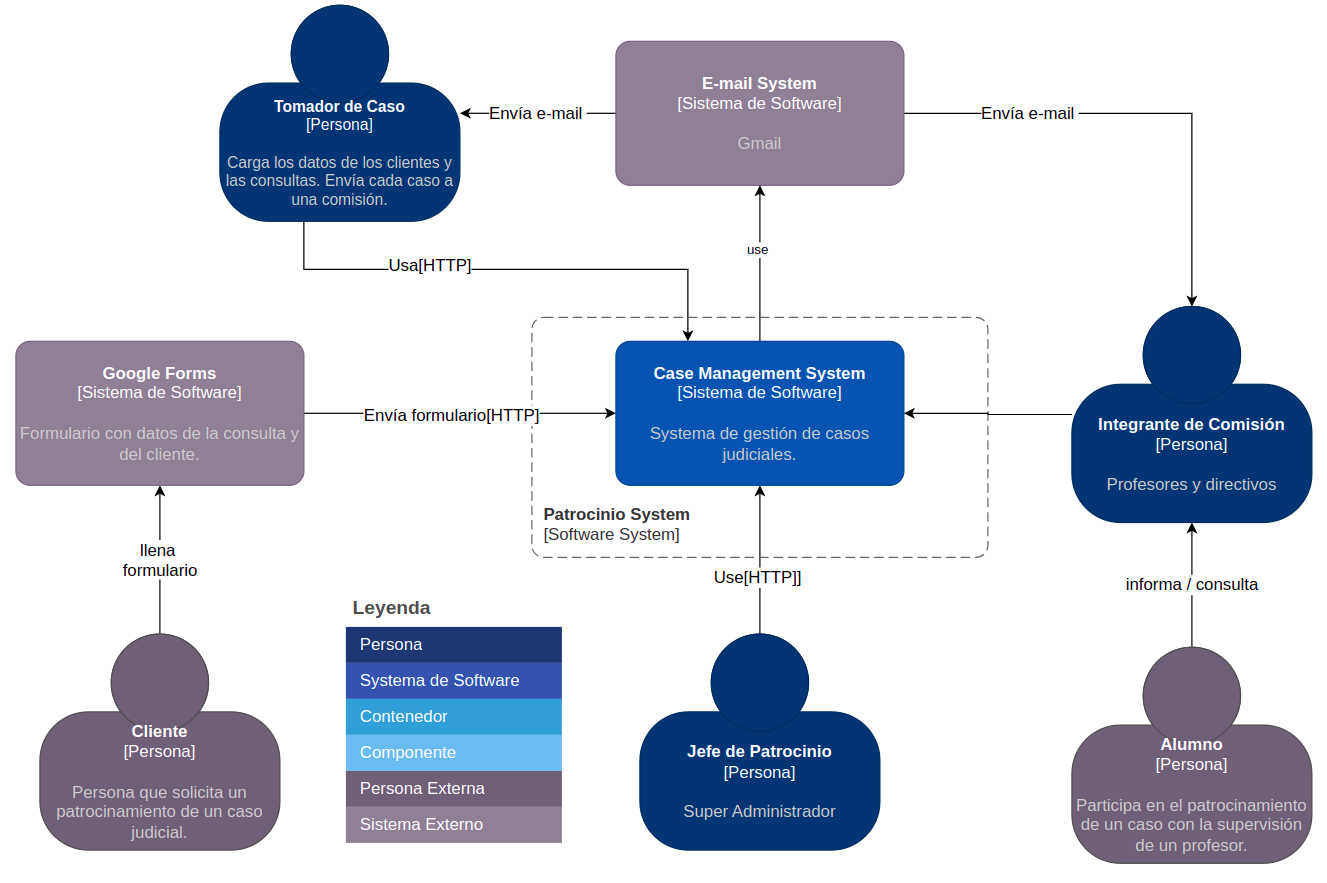
\includegraphics[width=1.1\linewidth]{fig/c4-1.png}
    \caption{Diagrama de Contexto C4}
    \label{fig:c4-01}
\end{figure}

\section{Acrónimos y Abreviaturas}
\label{sec:acronimos}

En el presente documento, se utilizan los siguientes acrónimos y abreviaturas:

\begin{table}[H]
    \centering
    \begin{tabular}{|c|p{10cm}|}
    \hline
         \textbf{Acrónimos} & \textbf{Descripción}\\
    \hline
         API & Interfaz de Programación de Aplicaciones (por sus siglas en inglés, \textit{Application Programming Interface})\\
    \hline
         HTTP & Protocolo de Transferencia de Hipertexto (por sus siglas en inglés, \textit{Hypertext Transfer Protocol})\\
    \hline
         IP & Protocolo de Internet (\textit{Internet Protocol})\\
    \hline
         JSON & Notación de Objetos de JavaScript (\textit{JavaScript Object Notation}) \\
    \hline
         REST & Transferencia de Estado Representacional (\textit{Representational State Transfer}) \\
    \hline
        DNS & Sistema de Nombres de Dominio (\textit{Domain Name System}) \\
    \hline
        SSL/TLS & Capa de Conexión Segura / Protocolo de Seguridad de la Capa de Transporte (\textit{Secure Sockets Layer / Transport Layer Security}) \\
    \hline
        SQL & Lenguaje de Consulta Estructurada (\textit{Structured Query Language}) \\
    \hline
        CORS & Intercambio de recursos de origen cruzado (\textit{Cross Origin Resource Sharing})\\
    \hline
         CSRF & Falsificación de Petición en Sitios Cruzados (\textit{Cross-Site Request Forgery}) \\
    \hline
         NIST & Instituto Nacional de Estándares y Tecnología (\textit{National Institute of Standards and Technology}) \\
    \hline
        CI & Integración Continua (\textit{Continuous Integration}) \\
    \hline
        CD & Entrega Continua (\textit{Continuous Delivery}) \\
    \hline
        UBA & Universidad de Buenos Aires \\
    \hline
        UNC & Universidad Nacional de Córdoba \\
    \hline
       ASGI & Interfaz de Puerta de Enlace Asíncrona del Servidor (\textit{Asynchronous Server Gateway Interface}) \\
    \hline
        WSGI & Interfaz de Puerta de Enlace del Servidor Web (\textit{Web Server Gateway Interface}) \\
    \hline
        
    \end{tabular}
    \caption{Lista de Acrónimos y Abreviaturas}
    \label{tab:my_label}
\end{table}
